%%%% fatec-article.tex, 2024/03/10

\documentclass[
  a4paper,%% Tamanho de papel: a4paper, letterpaper (^), etc.
  12pt,%% Tamanho de fonte: 10pt (^), 11pt, 12pt, etc.
  english,%% Idioma secundário (penúltimo) (>)
  brazilian,%% Idioma primário (último) (>)
]{article}

%% Pacotes utilizados
\usepackage[]{fatec-article}
\usepackage{float}
\usepackage{listings}
\usepackage[utf8]{inputenc}
\usepackage{minted}

\lstset{
  basicstyle=\ttfamily\small, 
  frame=single,              
  numbers=left,             
  numberstyle=\tiny,         
  breaklines=true 
  escapeinside={(*@}{@*)},    
  showstringspaces=false     
}

%% Início do documento
\begin{document}
\vspace{8cm}
\begin{center}
    \large \textbf{\title{ARTEFATOS DO PROJETO DE SOFTWARE}}
\end{center}

\maketitle

\break

\tableofcontents

\break


%exemplo da forma de organização das seções e subseções, você deverá adaptar o template para a realidade do seu projeto.

\section*{Banco de Dados}
\addcontentsline{toc}{section}{Banco de Dados}

    Para a implementação do sistema, foram desenvolvidos o Modelo Lógico(Figura 1) do banco de dados não-relacional do aplicativo, que inclui uma base de dados das imagens a serem analisadas pelo sistema, assim como uma base de dados dos clientes cadastrados e  o diagnóstico realizado pelo sistema, apontando quais espécies foram identificadas em uma determinada imagem.
    

\begin{figure}[H]
    \centering
    \caption{Modelo lógico- Banco NoSQL. }
    \label{fig:my_label}
    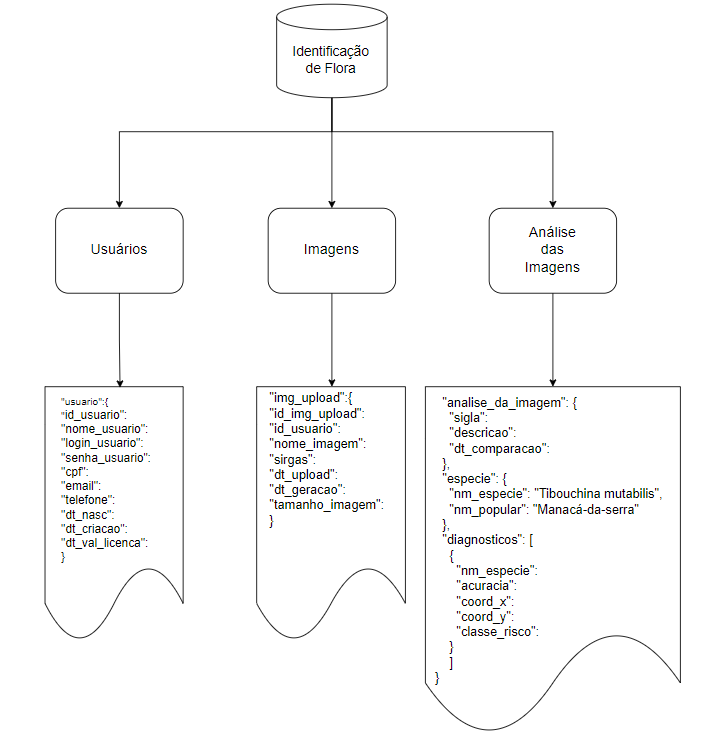
\includegraphics[width=.7\textwidth,keepaspectratio]{Logos/modelagem_nosql.png}
    \SourceOrNote{Fonte: Os Autores(2023)}
\end{figure}

\section*{Interface gráfica}
\addcontentsline{toc}{section}{Interface gráfica}

Utilizando a interface gráfica em Java, foi desenvolvido o sistema de Acesso do Usuário, bem como a funcionalidade do CRUD, onde é possível cadastrar,listar, alterar e excluir usuários do sistema.
Em busca de tornar o sistema intuitivo e de fácil acessibilidade ao usuário, foram feitas modificações nos protótipos. Com base nas teorias de processamento humano da informação.

\begin{figure}[H]
    \centering
    \caption{Tela de Login}
    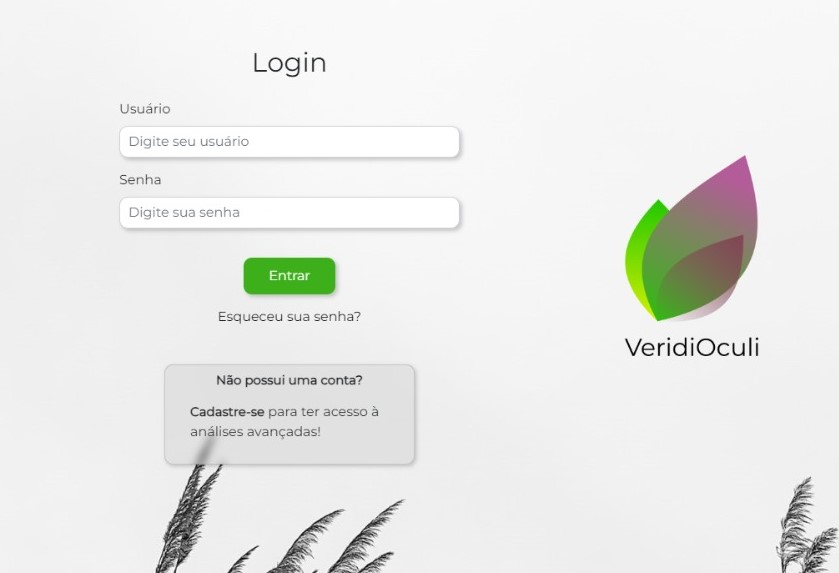
\includegraphics[width=.7\textwidth,keepaspectratio]{Logos/1.jpg}
    \SourceOrNote{Fonte: Os Autores(2023)}
    \label{fig:enter-label}
\end{figure}

A tela de login para o sistema web foi desenvolvido de acordo com os Padrões de Interface, como campo se senha após o campo de login, botão de confirmar em destaque e link para recuperação de senha, colocado em menor destaque.

\begin{figure}[H]
    \centering
    \caption{Tela de boas-vindas.}
    \includegraphics[width=.7\textwidth,keepaspectratio]{Logos/tela_pós-login.png}
    \SourceOrNote{Fonte: Os Autores(2023)}
    \label{fig:my_label}
\end{figure}


Após o login do usuário, a tela de boas vindas mostra ao usuário o preview das telas que irá visualizar no sistema. 

\begin{figure}[H]
    \centering
    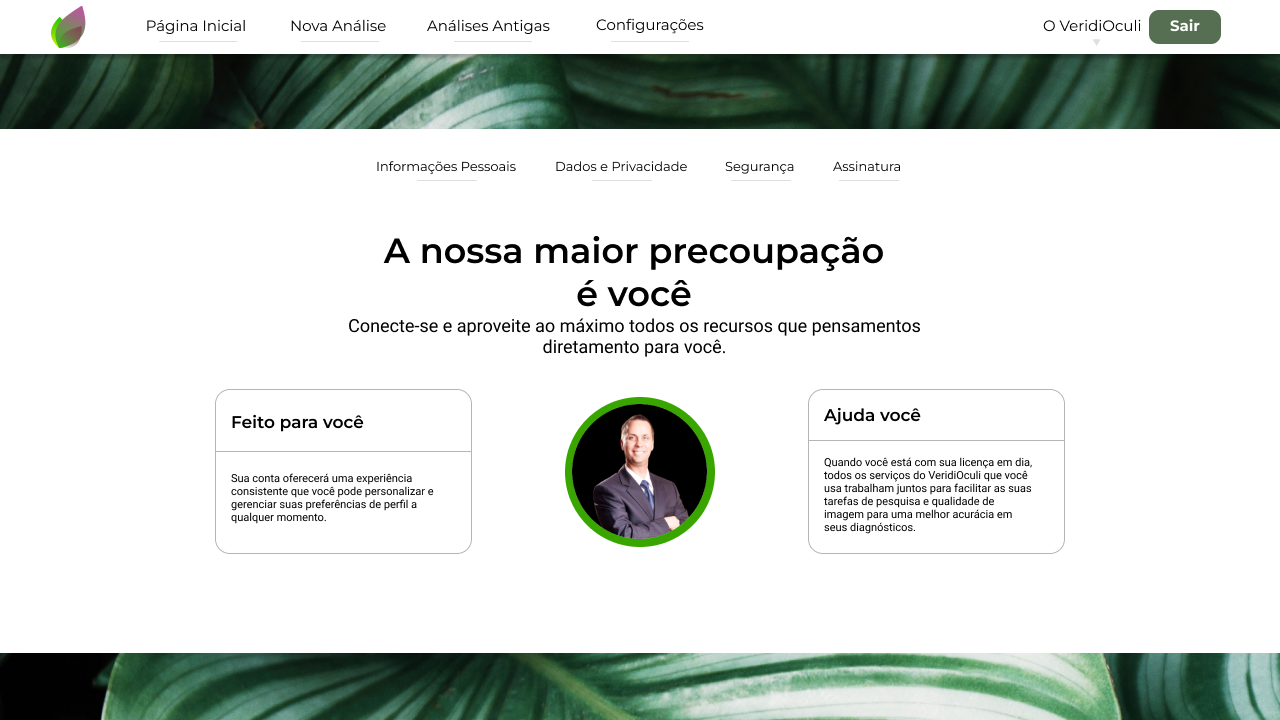
\includegraphics[width=.7\textwidth,keepaspectratio]{Logos/tela_configurações2.png}
    \caption{Tela de Configurações pessoais. Fonte: Os Autores}
    \label{fig:my_label}
\end{figure}

Na área de configurações de usuário, este será capaz de visualizar as proprias informações.


\begin{figure}[H]
    \centering
    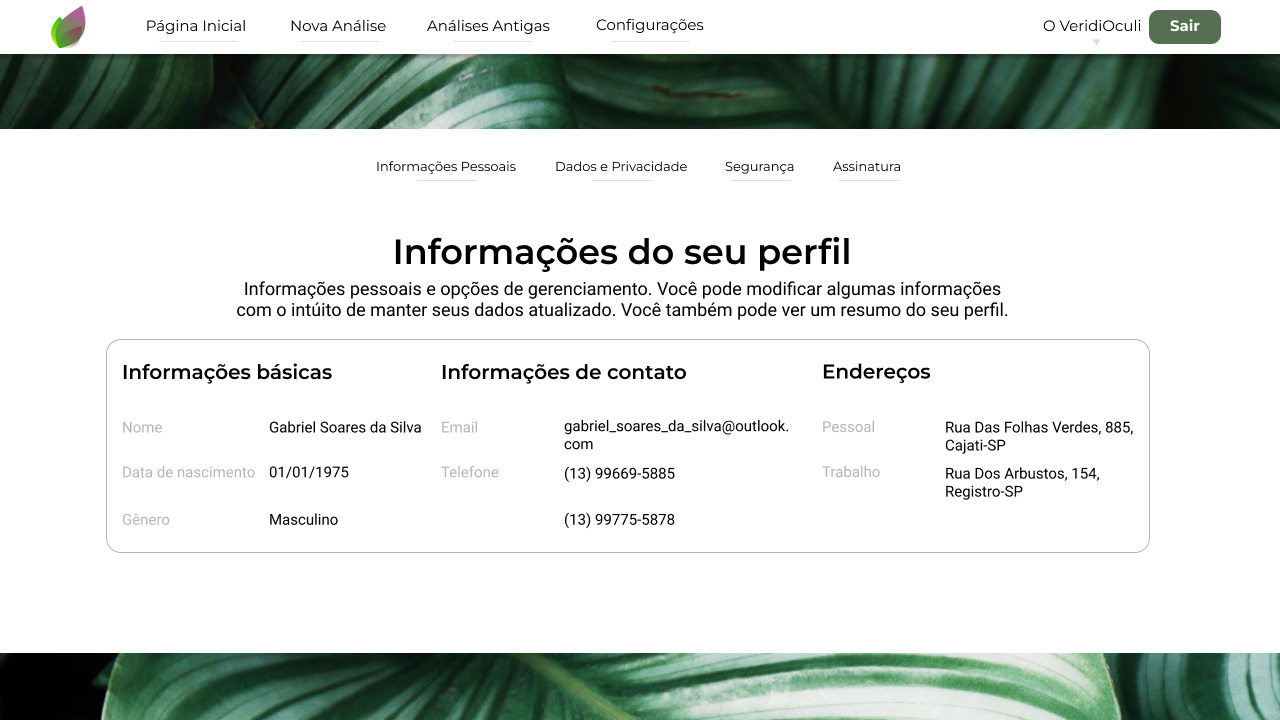
\includegraphics[width=.7\textwidth,keepaspectratio]{Logos/tela_configurações.png}
    \caption{Informações do usuário. Fonte: Os Autores}
    \label{fig:my_label}
\end{figure}


Será também capaz de adicionar e atualizar as informações de usuário.

\begin{figure}[H]
    \centering
    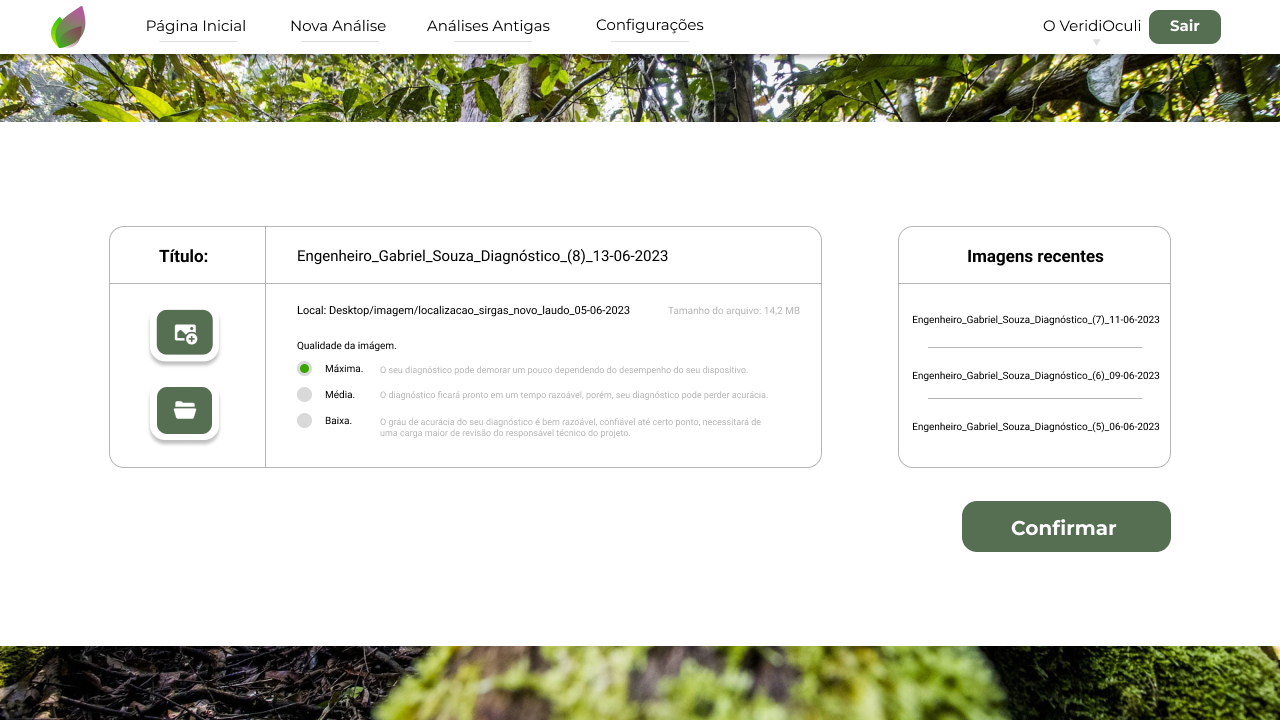
\includegraphics[width=\textwidth,keepaspectratio]{Logos/tela_subir_imagem.png}
    \caption{Tela do sistema de carregamento de imagens. Fonte: Os Autores}
    \label{fig:my_label}
\end{figure}

O protótipo de tela de carregamento de uma nova imagem para análise leva em conta a usabilidade e clareza nas informações do sistema.

\begin{figure}[H]
    \centering
    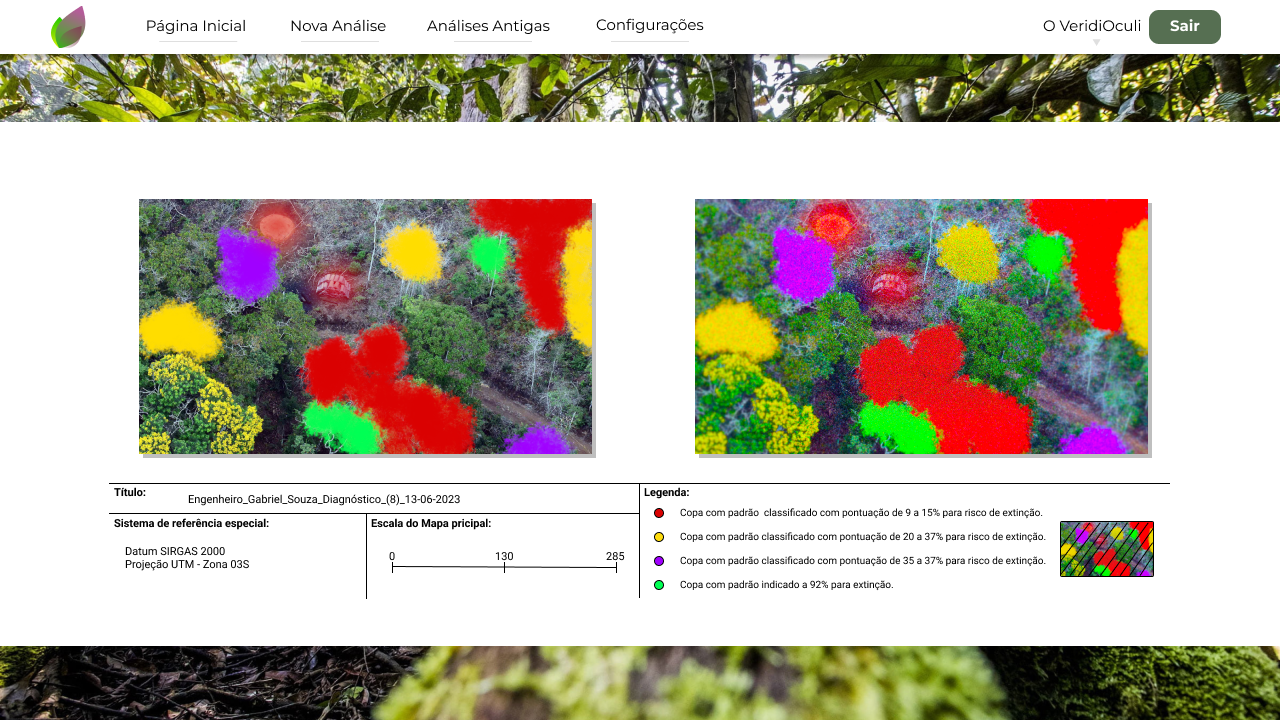
\includegraphics[width=\textwidth,keepaspectratio]{Logos/tela_diagnostico_detalhado_novo.png}
    \caption{Tela do sistema de análise. Fonte: Os Autores}
    \label{fig:my_label}
\end{figure}

Após a análise feita pelo modelo treinado, será possível buscar as espécies de árvores encontradas na foto.


\section*{Algoritmo de Ordenação}
\addcontentsline{toc}{section}{Algoritmo de Ordenação}
    

A análise de complexidade, realizada no presente trabalho para avaliar a eficiência do algorítmo de odenação QuickSort, nos mostrou que o melhor caso e o caso médio, temos que o número de iterações necessárias para chegar ao caso base, onde as partições têm tamanho 1, é log de n na base 2. Assim, a complexidade em termos de "k" é O$(\log n)$.\\

Substituindo essa complexidade na recorrência:\\

\begin{equation} 
\label{eu_eqn1}
        T(n) = 2T(k) + O(n) = 2O(\log n) + O(n) = O(\log n) + O(n)
\end{equation}

\begin{equation} 
    \label{eu_eqn}    
        T(n)= O(n \log n)
\end{equation}

Portanto, no melhor e caso médio, a complexidade do algoritmo QuickSort é O$(n \log n)$ (Equação 6)\\

A análise de recorrência para o pior caso, onde o número de iterações necessárias para chegar ao caso base é "n".

Substituindo "T(n-1)" por "T(k)" e considerando o número de iterações "n":\\

\begin{equation} 
    \label{eu_eqn}
        T(n) = T(n-1) + C + O(n) = T(k) + Cn + O
\end{equation}

\begin{equation} 
    \label{eu_eqn}
        T(n) = O(k) + Cn + O(n) = O(n) + O(n) + O(n) = O(n^2)
\end{equation}

\begin{equation} 
    \label{eu_eqn}
        T(n) = O(n^2)
\end{equation}

Portanto, no pior caso, a complexidade do algoritmo QuickSort é O$(n^2)$(Equação 11).

\section*{Modelo de Aprendizagem de Máquina}
    Para a implementação do sistema, foram desenvolvidos o Modelo Lógico(Figura 2) e o Modelo Físico(Anexo 1)do banco de dados não-relacional do aplicativo, que inclui uma base de dados das imagens a serem analisadas pelo sistema, assim como uma base de dados dos clientes cadastrados e  o diagnóstico realizado pelo sistema, apontando quais espécies foram identificadas em uma determinada imagem.  

    
    
\section*{Modelo de Aprendizagem FCNN}
\addcontentsline{toc}{section}{Modelo de Aprendizagem FCNN}

Para desenvolver o treinamento do modelo de aprendizagem profunda, foi utilizado o código em python, para classificar as imagens catalogadas no conjunto.

\begin{lstlisting}[language=Python, caption={Treinamento do modelo de aprendizagem profunda}]

import tensorflow as tf
from tensorflow.keras import layers, models
import matplotlib.pyplot as plt

import numpy as np
from sklearn.model_selection import KFold
import os

data_dir = 'img'

batch_size = 32
img_height = 170
img_width = 170
num_classes = len(os.listdir(data_dir))
num_folds = 10
epochs = 100

def create_model():
    model = models.Sequential()
    model.add(layers.Flatten(input_shape=(img_height, img_width, 3)))
    model.add(layers.Dense(512, activation='relu'))
    model.add(layers.Dense(256, activation='relu'))
    model.add(layers.Dense(num_classes, activation='softmax'))
    model.compile(optimizer='adam',
                  loss='sparse_categorical_crossentropy',
                  metrics=['accuracy'])
    return model

def load_data(file_paths, labels, img_height, img_width):
    images = []
    for file_path in file_paths:
        img = tf.keras.preprocessing.image.load_img(file_path, target_size=(img_height, img_width))
        img_array = tf.keras.preprocessing.image.img_to_array(img)
        images.append(img_array)
    return np.array(images), np.array(labels)

# Preparar os caminhos e labels
file_paths = []
labels = []
class_names = os.listdir(data_dir)
class_indices = {class_name: i for i, class_name in enumerate(class_names)}

for class_name in class_names:
    class_dir = os.path.join(data_dir, class_name)
    class_files = os.listdir(class_dir)
    file_paths.extend([os.path.join(class_dir, f) for f in class_files])
    labels.extend([class_indices[class_name]] * len(class_files))

# Inicializar KFold
kf = KFold(n_splits=num_folds, shuffle=True, random_state=42)


fold_accuracies = []
fold_no = 1
for train_index, val_index in kf.split(file_paths):
    print(f'Training fold {fold_no}...')
    
    train_files = [file_paths[i] for i in train_index]
    val_files = [file_paths[i] for i in val_index]
    train_labels = [labels[i] for i in train_index]
    val_labels = [labels[i] for i in val_index]
    
    x_train, y_train = load_data(train_files, train_labels, img_height, img_width)
    x_val, y_val = load_data(val_files, val_labels, img_height, img_width)
    
    # Normalizar os dados
    x_train = x_train / 255.0
    x_val = x_val / 255.0
    
    model = create_model()
    
    # Treinar o modelo
    history = model.fit(x_train, y_train, epochs=epochs, batch_size=batch_size, validation_data=(x_val, y_val))
    
    # Avaliar o modelo
    val_loss, val_acc = model.evaluate(x_val, y_val)
    print(f'Fold {fold_no} validation accuracy: {val_acc}')
    
    fold_accuracies.append(val_acc)
    fold_no += 1

print(f'Validation accuracies for each fold: {fold_accuracies}')
print(f'Mean validation accuracy: {np.mean(fold_accuracies)}')
print(f'Numero de classes: {num_classes}')
plt.plot(history.history['accuracy'], label='accuracy')
plt.plot(history.history['val_accuracy'], label='val_accuracy')
plt.xlabel('Epoch')
plt.ylabel('Accuracy')
plt.legend(loc='lower right')
plt.show()

\end{lstlisting}


\section*{Aplicação Mobile - Protótipo da aplicação}
\addcontentsline{toc}{section}{Aplicação Mobile}
\addcontentsline{toc}{subsection}{Protótipo da aplicação}

Desenvolvimento de aplicação mobile para geração e visualização de relatórios com base nas análises criadas com o modelo de identificação.

\begin{figure}[H]
    \centering
    \caption{Casos de Uso - Diagrama Mobile}
    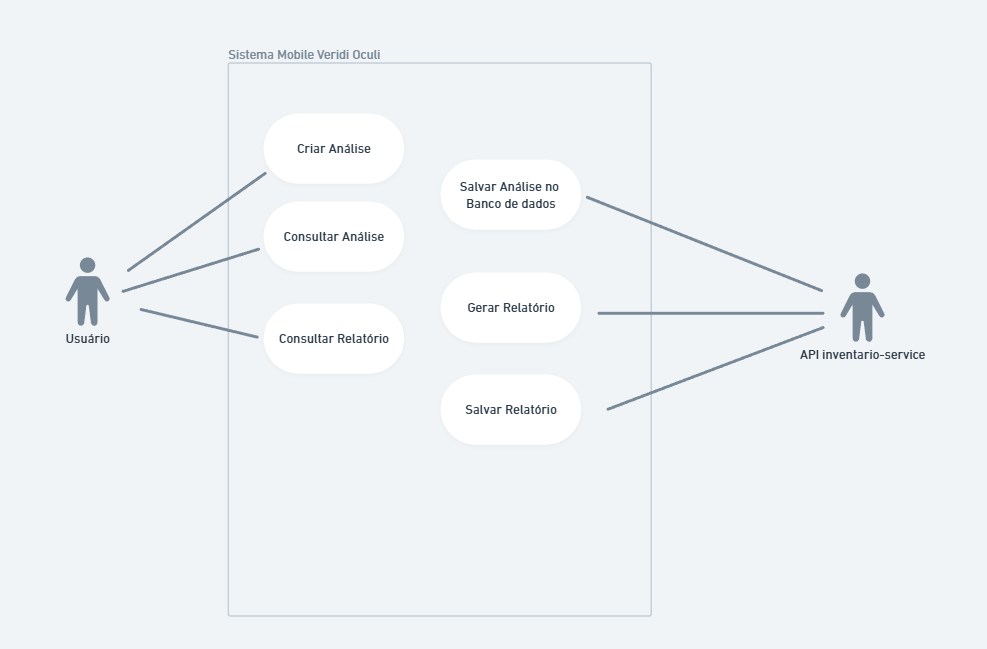
\includegraphics[width=.6\textwidth,keepaspectratio]{Logos/caso-de-uso-mobile.png}
    \SourceOrNote{Fonte: Os Autores(2024)}
    \label{fig:mobile1}
\end{figure}

O diagrama da figura 8, demonstra de forma simplificada os casos de uso da aplicação mobile.

\begin{figure}[H]
    \centering
    \caption{Tela de entrada - Mobile}
    
\includegraphics[width=.25\textwidth,keepaspectratio]{Logos/mobile-tela1.png}
    \SourceOrNote{Fonte: Os Autores(2024)}
    \label{fig:mobile1}
\end{figure}

A tela de entrada (figura 9), utiliza os mesmos padrões de tipografia e cores aplicados na versão web.

\begin{figure}[H]
    \centering
    \caption{Tela de Análises - Mobile}
    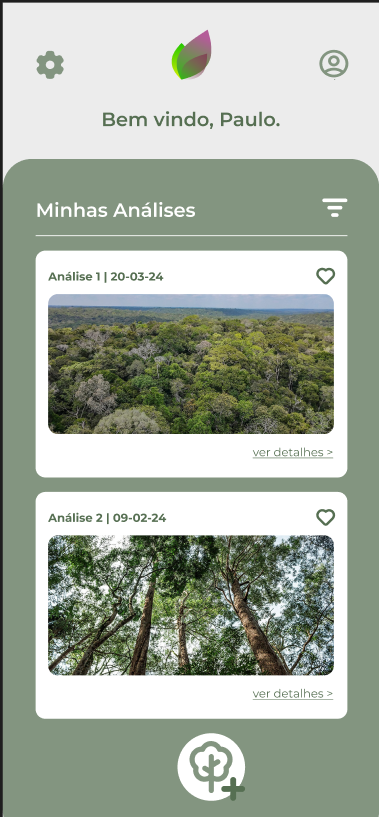
\includegraphics[width=.25\textwidth,keepaspectratio]{Logos/mobile-tela2.png}    \SourceOrNote{Fonte: Os Autores(2024)}
    \label{fig:mobile1}
\end{figure}

Feito o login, o usuário tem à sua disposição as análises realizadas anteriormente.

\begin{figure}[H]
    \centering
    \caption{Tela de Nova Análise - Mobile}
    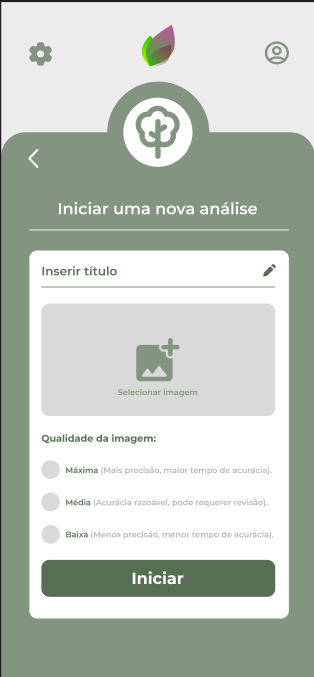
\includegraphics[width=.25\textwidth,keepaspectratio]{Logos/mobile-tela3.png}
    \SourceOrNote{Fonte: Os Autores(2024)}
    \label{fig:mobile1}
\end{figure}
O usuário pode também solicitar uma nova análise. Devendo para tal, inserir uma imagem e solicitar a identificação das espécies de árvores.
\begin{figure}[H]
    \centering
    \caption{Tela de Relatório - Mobile}
    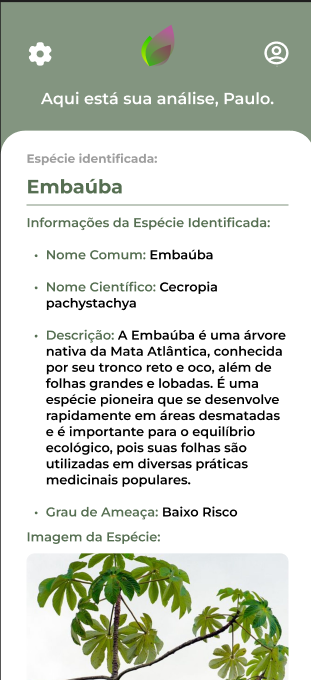
\includegraphics[width=.25\textwidth,keepaspectratio]{Logos/mobile-tela4.png}
    \SourceOrNote{Fonte: Os Autores(2024)}
    \label{fig:mobile1}
\end{figure}

Ao selecionar uma análise já processada, será disponibilizado o relatório de identificação das espécies encontradas na imagem disponibilizada pelo usuário. Nele constará informações sobre a espécie encontrada, e as marcações onde foram identificadas as espécies e outras informações como acurácia e posição na foto.

\subsection*{API para comunicação com recursos em nuvem}
\addcontentsline{toc}{subsection}{API para comunicação com recursos em nuvem}

Para fazer a comunicação com os recursos em nuvem como banco de dados, Storage Services e API generativa de textos, foi desenvolvido uma API em Python, hospedada em um EC2 (Elastic Computing Cloud) na AWS.

\begin{lstlisting}[language=Python, caption={API para gera\c{c}\~ao de relat\'{o}rios e intera\c{c}\~ao com S3}]

    import boto3
    import json
    import openai
    from flask import Blueprint, jsonify, request
    from dotenv import load_dotenv
    import os
    from app.services.genAnalise import genAnalise
    from app.services.s3_service import fetch_json_data
    
    load_dotenv()
    bp = Blueprint('analysis', __name__)
    
    # key = "analise01.json"
    s3 = boto3.client(
        's3',
        aws_access_key_id=os.getenv("AWS_ACCESS_KEY_ID"),
        aws_secret_access_key=os.getenv("AWS_SECRET_ACCESS_KEY")
    )

    openai.api_key = os.getenv("OPENAI_API_KEY")
    BUCKET_ANALISES = os.getenv("BUCKET_ANALISES")
    BUCKET_RELATORIO = os.getenv("BUCKET_RELATORIO")
    BUCKET_IMAGENS = os.getenv("BUCKET_IMAGENS")
    
    def save_report_to_bucket(bucket_name, key, content):
        """Salvar o relat\'{o}rio gerado no bucket S3"""
        s3.put_object(Bucket=bucket_name, Key=key, Body=json.dumps(content))
    
    @bp.route('/generate-report/<analysis_key>', methods=['POST'])
    def generate_report(analysis_key):
        """Gera o relat\'{o}rio com base em uma an\'{a}lise."""
        try:
            # 1. Buscar a an\'{a}lise no bucket de an\'{a}lises
            analysis_data = fetch_json_data(BUCKET_ANALISES, analysis_key)
    
            # 2. Obter a URL da imagem associada
            image_id = analysis_data.get('image_details', {}).get('image_id', '')
            image_url = f"https://{BUCKET_IMAGENS}.s3.amazonaws.com/{image_id}"
    
            # 3. Gerar o relat\'{o}rio com a OpenAI API
            report = genAnalise(analysis_data, image_url)
            print(report)
            if report:
                # 4. Salvar o relat\'{o}rio no bucket de relat\'{o}rios
                report_key = f"report_{analysis_key.split('.')[0]}.json"
                save_report_to_bucket(BUCKET_RELATORIO, report_key, json.loads(report))
                return jsonify({"status": "success", "report_key": report_key}), 200
            else:
                return jsonify({"status": "error", "message": "Erro ao gerar relat\'{o}rio"}), 500
        except Exception as e:
            return jsonify({"status": "error", "message": str(e)}), 500
    
\end{lstlisting}

Esta API(Listing 2) cria métodos para que a aplicação mobile possa interagir com os recursos em nuvem, buscando e salvando documentos relacionados ao usuário.

\begin{lstlisting}[language=Python, caption={API para comunica\c{c}\~ao com AI generativa OpenAI}]

from openai import OpenAI
import json
import os
from dotenv import load_dotenv

load_dotenv()
client = OpenAI(api_key=os.environ.get("OPENAI_API_KEY"))

def genAnalise(analysis_data, image_url):
    print("Gera o relat\'{o}rio de invent\'{a}rio florestal usando a API do OpenAI.")
    print(analysis_data)
    try:
        prompt = f"""
        Crie um relat\'{o}rio de invent\'{a}rio florestal com base nos seguintes dados:

        - Dados da an\'{a}lise (resumo): {json.dumps(analysis_data, ensure_ascii=False, indent=2)[:1000]}...
        - Imagem associada: {image_url}

        Siga o seguinte modelo:
        - ID da An\'{a}lise
        - Data da An\'{a}lise
        - Localiza\c{c}\~ao (latitude e longitude)
        - Resumo das identifica\c{c}\~oes (alta, m\'{e}dia e baixa confian\c{c}a)
        - Detalhes dos pontos de identifica\c{c}\~ao (coordenadas e confian\c{c}a)
        """

        response = client.chat.completions.create(
            model="gpt-3.5-turbo",
            messages=[
                {"role": "system", "content": "Voc\^{e} \'{e} um assistente especializado em cria\c{c}\~ao de relat\'{o}rios."},
                {"role": "user", "content": prompt}]
        )

        if response and response.choices:
            return response.choices[0].message.content
        else:
            raise ValueError("Resposta inv\'{a}lida ou vazia da OpenAI API.")
    except Exception as e:
        print(f"Erro ao gerar relat\'{o}rio: {e}")
        return None
    
\end{lstlisting}
    
Esta segunda API (Listing 3) é utilizada para comunicação com a API generativa da OpenAi, para tornar os dados conseguidos através da análise, legíveis e de fácil compreensão pelo usuário.
        

\end{document}